% Options for packages loaded elsewhere
\PassOptionsToPackage{unicode}{hyperref}
\PassOptionsToPackage{hyphens}{url}
\PassOptionsToPackage{dvipsnames,svgnames,x11names}{xcolor}
%
\documentclass[
  letterpaper,
  DIV=11,
  numbers=noendperiod]{scrartcl}

\usepackage{amsmath,amssymb}
\usepackage{iftex}
\ifPDFTeX
  \usepackage[T1]{fontenc}
  \usepackage[utf8]{inputenc}
  \usepackage{textcomp} % provide euro and other symbols
\else % if luatex or xetex
  \usepackage{unicode-math}
  \defaultfontfeatures{Scale=MatchLowercase}
  \defaultfontfeatures[\rmfamily]{Ligatures=TeX,Scale=1}
\fi
\usepackage{lmodern}
\ifPDFTeX\else  
    % xetex/luatex font selection
\fi
% Use upquote if available, for straight quotes in verbatim environments
\IfFileExists{upquote.sty}{\usepackage{upquote}}{}
\IfFileExists{microtype.sty}{% use microtype if available
  \usepackage[]{microtype}
  \UseMicrotypeSet[protrusion]{basicmath} % disable protrusion for tt fonts
}{}
\makeatletter
\@ifundefined{KOMAClassName}{% if non-KOMA class
  \IfFileExists{parskip.sty}{%
    \usepackage{parskip}
  }{% else
    \setlength{\parindent}{0pt}
    \setlength{\parskip}{6pt plus 2pt minus 1pt}}
}{% if KOMA class
  \KOMAoptions{parskip=half}}
\makeatother
\usepackage{xcolor}
\setlength{\emergencystretch}{3em} % prevent overfull lines
\setcounter{secnumdepth}{-\maxdimen} % remove section numbering
% Make \paragraph and \subparagraph free-standing
\makeatletter
\ifx\paragraph\undefined\else
  \let\oldparagraph\paragraph
  \renewcommand{\paragraph}{
    \@ifstar
      \xxxParagraphStar
      \xxxParagraphNoStar
  }
  \newcommand{\xxxParagraphStar}[1]{\oldparagraph*{#1}\mbox{}}
  \newcommand{\xxxParagraphNoStar}[1]{\oldparagraph{#1}\mbox{}}
\fi
\ifx\subparagraph\undefined\else
  \let\oldsubparagraph\subparagraph
  \renewcommand{\subparagraph}{
    \@ifstar
      \xxxSubParagraphStar
      \xxxSubParagraphNoStar
  }
  \newcommand{\xxxSubParagraphStar}[1]{\oldsubparagraph*{#1}\mbox{}}
  \newcommand{\xxxSubParagraphNoStar}[1]{\oldsubparagraph{#1}\mbox{}}
\fi
\makeatother

\usepackage{color}
\usepackage{fancyvrb}
\newcommand{\VerbBar}{|}
\newcommand{\VERB}{\Verb[commandchars=\\\{\}]}
\DefineVerbatimEnvironment{Highlighting}{Verbatim}{commandchars=\\\{\}}
% Add ',fontsize=\small' for more characters per line
\usepackage{framed}
\definecolor{shadecolor}{RGB}{241,243,245}
\newenvironment{Shaded}{\begin{snugshade}}{\end{snugshade}}
\newcommand{\AlertTok}[1]{\textcolor[rgb]{0.68,0.00,0.00}{#1}}
\newcommand{\AnnotationTok}[1]{\textcolor[rgb]{0.37,0.37,0.37}{#1}}
\newcommand{\AttributeTok}[1]{\textcolor[rgb]{0.40,0.45,0.13}{#1}}
\newcommand{\BaseNTok}[1]{\textcolor[rgb]{0.68,0.00,0.00}{#1}}
\newcommand{\BuiltInTok}[1]{\textcolor[rgb]{0.00,0.23,0.31}{#1}}
\newcommand{\CharTok}[1]{\textcolor[rgb]{0.13,0.47,0.30}{#1}}
\newcommand{\CommentTok}[1]{\textcolor[rgb]{0.37,0.37,0.37}{#1}}
\newcommand{\CommentVarTok}[1]{\textcolor[rgb]{0.37,0.37,0.37}{\textit{#1}}}
\newcommand{\ConstantTok}[1]{\textcolor[rgb]{0.56,0.35,0.01}{#1}}
\newcommand{\ControlFlowTok}[1]{\textcolor[rgb]{0.00,0.23,0.31}{\textbf{#1}}}
\newcommand{\DataTypeTok}[1]{\textcolor[rgb]{0.68,0.00,0.00}{#1}}
\newcommand{\DecValTok}[1]{\textcolor[rgb]{0.68,0.00,0.00}{#1}}
\newcommand{\DocumentationTok}[1]{\textcolor[rgb]{0.37,0.37,0.37}{\textit{#1}}}
\newcommand{\ErrorTok}[1]{\textcolor[rgb]{0.68,0.00,0.00}{#1}}
\newcommand{\ExtensionTok}[1]{\textcolor[rgb]{0.00,0.23,0.31}{#1}}
\newcommand{\FloatTok}[1]{\textcolor[rgb]{0.68,0.00,0.00}{#1}}
\newcommand{\FunctionTok}[1]{\textcolor[rgb]{0.28,0.35,0.67}{#1}}
\newcommand{\ImportTok}[1]{\textcolor[rgb]{0.00,0.46,0.62}{#1}}
\newcommand{\InformationTok}[1]{\textcolor[rgb]{0.37,0.37,0.37}{#1}}
\newcommand{\KeywordTok}[1]{\textcolor[rgb]{0.00,0.23,0.31}{\textbf{#1}}}
\newcommand{\NormalTok}[1]{\textcolor[rgb]{0.00,0.23,0.31}{#1}}
\newcommand{\OperatorTok}[1]{\textcolor[rgb]{0.37,0.37,0.37}{#1}}
\newcommand{\OtherTok}[1]{\textcolor[rgb]{0.00,0.23,0.31}{#1}}
\newcommand{\PreprocessorTok}[1]{\textcolor[rgb]{0.68,0.00,0.00}{#1}}
\newcommand{\RegionMarkerTok}[1]{\textcolor[rgb]{0.00,0.23,0.31}{#1}}
\newcommand{\SpecialCharTok}[1]{\textcolor[rgb]{0.37,0.37,0.37}{#1}}
\newcommand{\SpecialStringTok}[1]{\textcolor[rgb]{0.13,0.47,0.30}{#1}}
\newcommand{\StringTok}[1]{\textcolor[rgb]{0.13,0.47,0.30}{#1}}
\newcommand{\VariableTok}[1]{\textcolor[rgb]{0.07,0.07,0.07}{#1}}
\newcommand{\VerbatimStringTok}[1]{\textcolor[rgb]{0.13,0.47,0.30}{#1}}
\newcommand{\WarningTok}[1]{\textcolor[rgb]{0.37,0.37,0.37}{\textit{#1}}}

\providecommand{\tightlist}{%
  \setlength{\itemsep}{0pt}\setlength{\parskip}{0pt}}\usepackage{longtable,booktabs,array}
\usepackage{calc} % for calculating minipage widths
% Correct order of tables after \paragraph or \subparagraph
\usepackage{etoolbox}
\makeatletter
\patchcmd\longtable{\par}{\if@noskipsec\mbox{}\fi\par}{}{}
\makeatother
% Allow footnotes in longtable head/foot
\IfFileExists{footnotehyper.sty}{\usepackage{footnotehyper}}{\usepackage{footnote}}
\makesavenoteenv{longtable}
\usepackage{graphicx}
\makeatletter
\newsavebox\pandoc@box
\newcommand*\pandocbounded[1]{% scales image to fit in text height/width
  \sbox\pandoc@box{#1}%
  \Gscale@div\@tempa{\textheight}{\dimexpr\ht\pandoc@box+\dp\pandoc@box\relax}%
  \Gscale@div\@tempb{\linewidth}{\wd\pandoc@box}%
  \ifdim\@tempb\p@<\@tempa\p@\let\@tempa\@tempb\fi% select the smaller of both
  \ifdim\@tempa\p@<\p@\scalebox{\@tempa}{\usebox\pandoc@box}%
  \else\usebox{\pandoc@box}%
  \fi%
}
% Set default figure placement to htbp
\def\fps@figure{htbp}
\makeatother

\KOMAoption{captions}{tableheading}
\makeatletter
\@ifpackageloaded{caption}{}{\usepackage{caption}}
\AtBeginDocument{%
\ifdefined\contentsname
  \renewcommand*\contentsname{Table of contents}
\else
  \newcommand\contentsname{Table of contents}
\fi
\ifdefined\listfigurename
  \renewcommand*\listfigurename{List of Figures}
\else
  \newcommand\listfigurename{List of Figures}
\fi
\ifdefined\listtablename
  \renewcommand*\listtablename{List of Tables}
\else
  \newcommand\listtablename{List of Tables}
\fi
\ifdefined\figurename
  \renewcommand*\figurename{Figure}
\else
  \newcommand\figurename{Figure}
\fi
\ifdefined\tablename
  \renewcommand*\tablename{Table}
\else
  \newcommand\tablename{Table}
\fi
}
\@ifpackageloaded{float}{}{\usepackage{float}}
\floatstyle{ruled}
\@ifundefined{c@chapter}{\newfloat{codelisting}{h}{lop}}{\newfloat{codelisting}{h}{lop}[chapter]}
\floatname{codelisting}{Listing}
\newcommand*\listoflistings{\listof{codelisting}{List of Listings}}
\makeatother
\makeatletter
\makeatother
\makeatletter
\@ifpackageloaded{caption}{}{\usepackage{caption}}
\@ifpackageloaded{subcaption}{}{\usepackage{subcaption}}
\makeatother

\usepackage{bookmark}

\IfFileExists{xurl.sty}{\usepackage{xurl}}{} % add URL line breaks if available
\urlstyle{same} % disable monospaced font for URLs
\hypersetup{
  pdftitle={Critical Computational Geographies -- Measures of Segregation},
  pdfauthor={Nathan Alexander, PhD},
  colorlinks=true,
  linkcolor={blue},
  filecolor={Maroon},
  citecolor={Blue},
  urlcolor={Blue},
  pdfcreator={LaTeX via pandoc}}


\title{Critical Computational Geographies -- Measures of Segregation}
\usepackage{etoolbox}
\makeatletter
\providecommand{\subtitle}[1]{% add subtitle to \maketitle
  \apptocmd{\@title}{\par {\large #1 \par}}{}{}
}
\makeatother
\subtitle{Technical Appendix}
\author{Nathan Alexander, PhD}
\date{}

\begin{document}
\maketitle


\section{Introduction}\label{introduction}

I outline the technical documentation for the Fall 2025
\href{quant-shop.github.io}{Quantitative Histories Workshop} series on
\href{https://quant-shop.github.io/events.html\#fall}{\emph{Critical
Computational Geographies}}. In this particular section, we focus on
questions about indicators used to quantify segregation. This section is
part of a long-term project of the Quantitative Histories Workshop
focused on exploring the dynamic features of context in probability and
high-dimensional data.

\subsection{Conceptual Model}\label{conceptual-model}

High-dimensional data are characterized by the relationship between the
data's dimensions (the number of features) and the data sample (number
of observations). In an ideal interdisciplinary model that is informed
by the various fields of human development, there is a potential to
understand how the number of data features relate to the sample, and
what methodological selections are used to characterize the set of
indicators used in a mathematical model.

We will use U.S. census data to consider a measure of dissimilarity and
spatial maps to: (1) observe land and coverings of different variables
that quantify race, and (2) engage in assessing the various spatial
conditions that inform racial isolation, or a series of dividing walls
that separate one group from another group
(\href{https://plus.maths.org/content/dividing-walls-topology-and-topography-i}{Short,
2011}).

\subsubsection{Example: A Theory of Dividing
Walls}\label{example-a-theory-of-dividing-walls}

\begin{figure}[H]

{\centering \pandocbounded{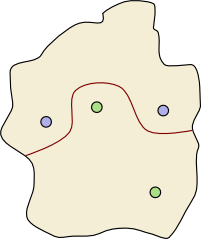
\includegraphics[keepaspectratio]{img/figureb.png}}

}

\caption{A sample dividing wall separating one group from another group}

\end{figure}%

Short's (2011) \emph{Dividing Wall's Theorem} presents a simplified
topological equivalence to consider the conditions of segregation and
isolation when a population of individuals are split into two groups. In
the current instance, we will examine dissimilarity in a measure of
Black and non-Black populations over some geographical area, \(G\).

\begin{figure}[H]

{\centering \pandocbounded{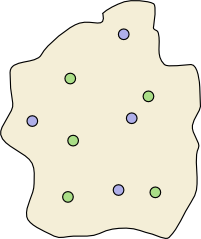
\includegraphics[keepaspectratio]{img/figurec.png}}

}

\caption{Is there a dividing wall?}

\end{figure}%

\begin{quote}
\emph{Theorem 1.} Given any configuration of blue and green towns, there
is a dividing wall that separates blue towns from green towns.
\end{quote}

\begin{figure}[H]

{\centering \pandocbounded{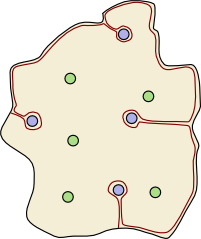
\includegraphics[keepaspectratio]{img/figured.png}}

}

\caption{Visual proof of Short's (2001) Dividing Wall's Theorem}

\end{figure}%

In the conceptual analysis above, there were only two tracts present and
they completely segregated the two groups by the dividing wall. This
conceptual model is a base example: two groups, two tracks, complete
segregation.

\subsection{Computational Model}\label{computational-model}

The index of dissimilarity will be used to quantify the evenness with
which Black residents are distributed relative to other non-Black racial
groups across census tracts. Our current analysis builds on the
perspectives that these base measures may be foundational in
understanding and quantifying the dimensions of antiblackness in
high-dimensional data sources.

The index of dissimilarity, \(D\), is a demographic measure of the
evenness with which two groups are distributed across geographic units
within a larger geographical area. The measure quantifies the percentage
of one group that would need to relocate to achieve an even distribution
across all units in the geographical area. A value of \(D = 0\)
corresponds to complete integration, while \(D = 1\) indicates complete
segregation.

\[
D = \frac{1}{2} \sum_{i=1}^N \left| \dfrac{a_i}{A} - \dfrac{b_i}{B} \right|
\]

where

\begin{itemize}
\tightlist
\item
  \(N\) is the number of geographic units (e.g., census tracts),
\item
  \(a_i\) is the population of group A (e.g., Black residents) in unit
  \(i\),
\item
  \(A\) is the total population of group A,
\item
  \(b_i\) is the population of group B (e.g., non-Black residents) in
  unit \(i\),
\item
  \(B\) is the total population of group B.
\end{itemize}

\(D\) measures the unevenness or lack of even distribution between Black
and non-Black residents across the geographical units of a region \(G\).
The index \(D\) takes on values from \(0\) (complete integration) to
\(1\) (complete segregation) and represents the fraction of a group's
population that would need to relocate to achieve an even spatial
distribution. For example, if \(D = 0.60\), 60\% of one group would need
to move to different areas to achieve integration.

\subsubsection{Example: Hypothetical City Census
Tracts}\label{example-hypothetical-city-census-tracts}

We can build on the hypothetical example provided by
\href{https://coascenters.howard.edu/dissimilarity-index-tutorial}{Dr.~Rodney
Green (n.d.)} where he offers a tutorial of the dissimilarity index. In
the example, Green (n.d.) models five tracts containing between 10 and
200 residents. I recreate Green's example below:

Consider the following hypothetical city with five census tracts.

\emph{Table 1: Hypothetical distribution of Black (\(B\)) and White
(\(W\)) households across five census tracts with intermediate
calculations toward the Index of Dissimilarity.}

\begin{longtable}[]{@{}
  >{\raggedright\arraybackslash}p{(\linewidth - 10\tabcolsep) * \real{0.0875}}
  >{\raggedright\arraybackslash}p{(\linewidth - 10\tabcolsep) * \real{0.1375}}
  >{\raggedright\arraybackslash}p{(\linewidth - 10\tabcolsep) * \real{0.1375}}
  >{\raggedright\arraybackslash}p{(\linewidth - 10\tabcolsep) * \real{0.1625}}
  >{\raggedright\arraybackslash}p{(\linewidth - 10\tabcolsep) * \real{0.1625}}
  >{\raggedright\arraybackslash}p{(\linewidth - 10\tabcolsep) * \real{0.3125}}@{}}
\toprule\noalign{}
\begin{minipage}[b]{\linewidth}\raggedright
Tract
\end{minipage} & \begin{minipage}[b]{\linewidth}\raggedright
\(b_i\)
\end{minipage} & \begin{minipage}[b]{\linewidth}\raggedright
\(w_i\)
\end{minipage} & \begin{minipage}[b]{\linewidth}\raggedright
\(\dfrac{b_i}{B = 300}\)
\end{minipage} & \begin{minipage}[b]{\linewidth}\raggedright
\(\dfrac{w_i}{W = 500}\)
\end{minipage} & \begin{minipage}[b]{\linewidth}\raggedright
absolute difference
\end{minipage} \\
\midrule\noalign{}
\endhead
\bottomrule\noalign{}
\endlastfoot
1 & \(b_1 = 50\) & \(w_1 = 10\) & 0.1667 & 0.0200 & 0.1467 \\
2 & \(b_2 = 200\) & \(w_2 = 40\) & 0.6667 & 0.0800 & 0.5867 \\
3 & \(b_3 = 10\) & \(w_3 = 100\) & 0.0333 & 0.2000 & 0.1667 \\
4 & \(b_4 = 30\) & \(w_4 = 200\) & 0.1000 & 0.4000 & 0.3000 \\
5 & \(b_5 = 10\) & \(w_5 = 150\) & 0.0333 & 0.3000 & 0.2667 \\
& & & & & \(\sum =\) 1.47 \\
\end{longtable}

where,

\begin{itemize}
\tightlist
\item
  \(B = \sum b_i = 300\) is the total number of Black households,
\item
  \(W = \sum w_i = 500\) is the total number of White households.
\end{itemize}

In Green's example, the index of dissimilarity \(D\) is computed as
follows:

\[
D = \frac{1}{2} \sum_{i=1}^{\textcolor{red}{N}}  \left| \frac{b_i}{B} - \frac{w_i}{W} \right|
\]

with \(N=5\) we update our index:

\[
D = \frac{1}{2} \sum_{i=1}^{\textcolor{red}{5}} \left| \frac{b_i}{B} - \frac{w_i}{W} \right|
\]

we then update our population, where \(B = \sum b_i = 300\) and
\(W = \sum w_i = 500\).

\[
D = \frac{1}{2} \sum_{i=1}^{5} \left| \frac{b_i}{\textcolor{blue}{B = 300}} - \frac{w_i}{\textcolor{blue}{W = 500}} \right|
\]

So we now have:

\[
D = \frac{1}{2} \sum_{i=1}^5 \left| \frac{b_i}{300} - \frac{w_i}{500} \right| 
\]

We then subsitute our values in the expansion, starting with total
populations:

\[
D = \frac{1}{2} \left( 
\left| \frac{b_1}{300} - \frac{w_1}{500} \right| +
\left| \frac{b_2}{300} - \frac{w_2}{500} \right| +
\left| \frac{b_3}{300} - \frac{w_3}{500} \right| +
\left| \frac{b_4}{300} - \frac{w_4}{500} \right| +
\left| \frac{b_5}{300} - \frac{w_5}{500} \right|
\right )
\]

and then values from each neighborhood in the numerators:

\[
D = \frac{1}{2} \left(
\left| \frac{50}{300} - \frac{10}{500} \right| +
\left| \frac{200}{300} - \frac{40}{500} \right| +
\left| \frac{10}{300} - \frac{100}{500} \right| +
\left| \frac{30}{300} - \frac{200}{500} \right| +
\left| \frac{10}{300} - \frac{150}{500} \right|
\right)
\]

or, more succinctly:

\[
D = \frac{1}{2} \sum_{i=1}^5 \left| \frac{b_i}{B} - \frac{w_i}{W} \right| = \frac{1}{2} (0.1467 + 0.5867 + 0.1667 + 0.3000 + 0.2667) = 0.7334
\]

Green notes that 73.3 percent of either Black households would need to
relocate to another tract to achieve an even distribution. In his
discussion, Green first holds the White population constant in each
tract and points to
\href{https://www.eeoc.gov/statutes/title-vii-civil-rights-act-1964}{Title
VII of the Civil Rights Acts} when ``White neighborhoods became
available to Black households that previously had been constrained, by
law and extra-legal practices, to live in densely populated inner
cities'' (Green, n.d.). He then presents the example when there is a
swap to achieve racial parity across the census tracts. We modify the
model and diverge from Green's example toward another end, based on our
theoretical framework centered on segregation as one measure of
antiblackness.

\section{Research Question}\label{research-question}

How segregated are Black residents from other racial groups across
census tracts, as quantified by the index of dissimilarity, \(D\)?

\section{Data and Methods}\label{data-and-methods}

For this analysis, we will use data from the U.S. Census Bureau, which
includes information from the
\href{https://www.census.gov/programs-surveys/decennial-census.html}{decennial
census} and the
\href{https://www.census.gov/programs-surveys/acs.html}{American
Community Survey (ACS)} 5-year estimates.

There are some essential items needed to generate our maps and begin our
investigations. First, please make sure you have requested and stored
your \href{https://api.census.gov/data/key_signup.html}{Census API key}
for easy access. Next, you will need to get set up in R and the
\href{https://www.google.com/url?sa=t&source=web&rct=j&opi=89978449&url=https://posit.co/products/open-source/rstudio/&ved=2ahUKEwjHgNqLouWPAxX8FlkFHS1VCBoQFnoECBkQAQ&usg=AOvVaw2_EHeeDq6zN5gnktCVwGMF}{R
and the RStudio IDE} (or \href{https://posit.cloud/}{Posit Cloud}) and
load the necessary packages and libraries.

Finally, you will need to select a geographical area that you would like
to explore.

\begin{Shaded}
\begin{Highlighting}[]
\CommentTok{\# Install packages as needed}
\CommentTok{\# install.packages(c("tidycensus", "tidyverse", "mapview", "mapgl", "quarto"))}

\CommentTok{\# Load your Census}
\CommentTok{\#CENSUS\_API\_KEY=\textquotesingle{}your\_api\_key\textquotesingle{}}

\CommentTok{\# Load necessary libraries}
\FunctionTok{library}\NormalTok{(tidycensus)}
\FunctionTok{library}\NormalTok{(dplyr)}
\FunctionTok{library}\NormalTok{(ggplot2)}
\FunctionTok{library}\NormalTok{(sf)}
\FunctionTok{library}\NormalTok{(viridis)}
\FunctionTok{library}\NormalTok{(scales)}
\end{Highlighting}
\end{Shaded}

\subsection{Model Assumptions}\label{model-assumptions}

We will suppose that a geographical area, \(G\), consists of \(N\)
tracts such that
\[G = \{g_1, g_2, g_3, ...g_N\} = \{tract_1, tract_2, tract_3, ..., tract_N\}\]

where,

\begin{itemize}
\tightlist
\item
  \(G\) is the set of census tracts that fully cover a geographical
  area,
\item
  \(g_i\) is the \(i\)-th tract such that \(g_1 =\) tract 1, \(g_2 =\)
  tract 2, \(g_3 =\) tract 3, \ldots,
\item
  \(N\) is the number of geographic units (e.g., census tracts)
\end{itemize}

We assume that \(G\) can be modeled by discrete data over a minimum
population of \(n\) individuals, where there is at least one individual
in each unit, i.e., \(n \ge N\) (so that no unit in \(G\) is empty,
i.e., all geographical units contain at least one individual).

We also modify the group meanings in the model to attend to the
theoretical framework centered on measures of segregation that support
our continued understanding of antiblackness. Specifically, we have:

\[
\hat{D} = \frac{1}{2} \sum_{i=1}^N \left| \dfrac{b_i}{b} - \dfrac{o_i}{O} \right|
\]

where

\begin{itemize}
\tightlist
\item
  \(N\) is the number of geographic units (e.g., census tracts),
\item
  \(b_i\) is the population of Black residents in unit \(i\),
\item
  \(B\) is the total population of Black residents,
\item
  \(o_i\) is the population of non-Black (other) residents in unit
  \(i\),
\item
  \(O\) is the total population of non-Black (other) residents.
\end{itemize}

\section{Findings}\label{findings}

\subsection{DC}\label{dc}

Given the structure of DC, we use \texttt{geography\ =\ "tract"} on the
variable \texttt{B02001\_003} for Black alone.

\begin{Shaded}
\begin{Highlighting}[]
\NormalTok{dc\_tracts }\OtherTok{\textless{}{-}} \FunctionTok{get\_acs}\NormalTok{(}
  \AttributeTok{geography =} \StringTok{"tract"}\NormalTok{,}
  \AttributeTok{variables =} \FunctionTok{c}\NormalTok{(}\AttributeTok{black =} \StringTok{"B02001\_003"}\NormalTok{, }\CommentTok{\# Black/African American population alone}
                \AttributeTok{total =} \StringTok{"B01001\_001"} \CommentTok{\# Total population}
\NormalTok{  ),}
  \AttributeTok{state =} \StringTok{"DC"}\NormalTok{,}
  \AttributeTok{year =} \DecValTok{2023}\NormalTok{,}
  \AttributeTok{geometry =}\NormalTok{ T,}
  \AttributeTok{output =} \StringTok{"wide"}
\NormalTok{)}
\end{Highlighting}
\end{Shaded}

We can then look at the first few and last few rows of our estimates.

\begin{Shaded}
\begin{Highlighting}[]
\NormalTok{dc\_tracts }\OtherTok{\textless{}{-}}\NormalTok{ dc\_tracts }\SpecialCharTok{\%\textgreater{}\%} 
  \FunctionTok{mutate}\NormalTok{(}\AttributeTok{nonblackE =}\NormalTok{ totalE }\SpecialCharTok{{-}}\NormalTok{ blackE) }\SpecialCharTok{\%\textgreater{}\%} 
  \FunctionTok{select}\NormalTok{(GEOID, blackE, nonblackE, totalE)}
\end{Highlighting}
\end{Shaded}

We'll then plot our data to get an initial visual of the variable.

\begin{Shaded}
\begin{Highlighting}[]
\FunctionTok{ggplot}\NormalTok{(dc\_tracts) }\SpecialCharTok{+}
  \FunctionTok{geom\_sf}\NormalTok{(}\FunctionTok{aes}\NormalTok{(}\AttributeTok{fill =}\NormalTok{ blackE)) }\SpecialCharTok{+}
  \FunctionTok{scale\_fill\_viridis\_c}\NormalTok{(}\AttributeTok{option =} \StringTok{"magma"}\NormalTok{, }
                       \AttributeTok{na.value =} \StringTok{"grey50"}\NormalTok{,}
                       \AttributeTok{labels =}\NormalTok{ comma) }\SpecialCharTok{+}
  \FunctionTok{labs}\NormalTok{(}\AttributeTok{title =} \StringTok{"Estimated Black Population by Census Tract in DC (2023)"}\NormalTok{,}
       \AttributeTok{fill =} \StringTok{"Population"}\NormalTok{) }\SpecialCharTok{+}
  \FunctionTok{theme\_minimal}\NormalTok{()}
\end{Highlighting}
\end{Shaded}

\pandocbounded{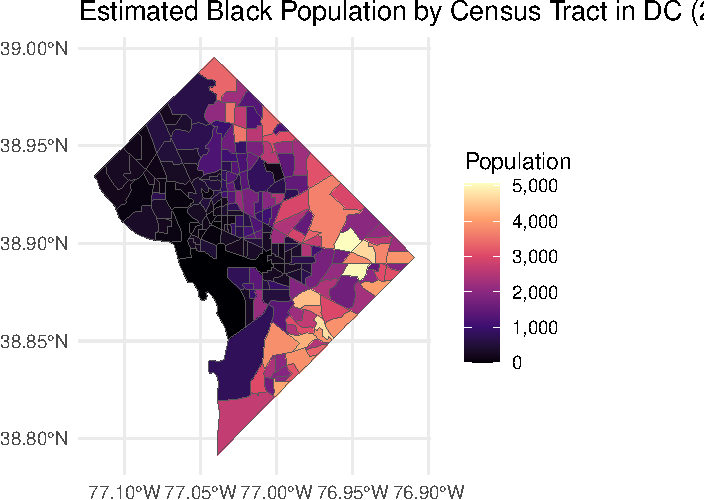
\includegraphics[keepaspectratio]{crit-comp-geo-pt1_files/figure-pdf/unnamed-chunk-4-1.pdf}}

And the data for non-Black individuals.

\begin{Shaded}
\begin{Highlighting}[]
\FunctionTok{ggplot}\NormalTok{(dc\_tracts) }\SpecialCharTok{+}
  \FunctionTok{geom\_sf}\NormalTok{(}\FunctionTok{aes}\NormalTok{(}\AttributeTok{fill =}\NormalTok{ nonblackE)) }\SpecialCharTok{+}
  \FunctionTok{scale\_fill\_viridis\_c}\NormalTok{(}\AttributeTok{option =} \StringTok{"magma"}\NormalTok{, }
                       \AttributeTok{na.value =} \StringTok{"grey50"}\NormalTok{,}
                       \AttributeTok{labels =}\NormalTok{ comma) }\SpecialCharTok{+}
  \FunctionTok{labs}\NormalTok{(}\AttributeTok{title =} \StringTok{"Estimated Non{-}Black Population by Census Tract in DC (2023)"}\NormalTok{,}
       \AttributeTok{fill =} \StringTok{"Population"}\NormalTok{) }\SpecialCharTok{+}
  \FunctionTok{theme\_minimal}\NormalTok{()}
\end{Highlighting}
\end{Shaded}

\pandocbounded{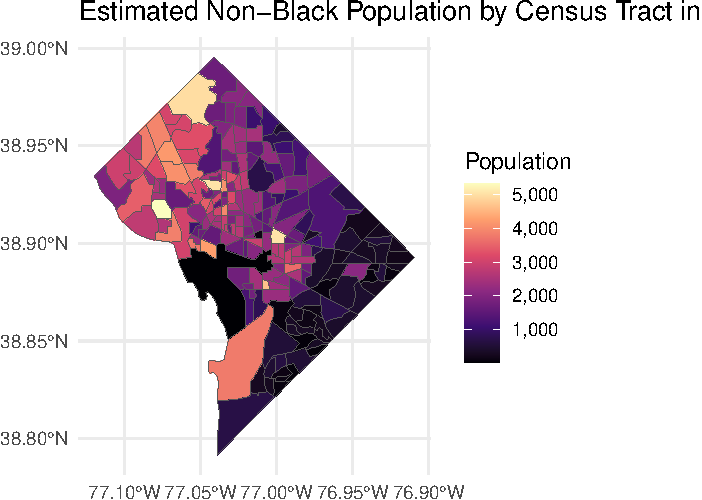
\includegraphics[keepaspectratio]{crit-comp-geo-pt1_files/figure-pdf/unnamed-chunk-5-1.pdf}}

\begin{center}\rule{0.5\linewidth}{0.5pt}\end{center}

Now that we know our maps feature is working, we begin our
investigation.

We first make a \texttt{dc\_black\_pop} data frame.

\begin{Shaded}
\begin{Highlighting}[]
\CommentTok{\# Get Black population by tract in DC}
\NormalTok{dc\_black\_pop }\OtherTok{\textless{}{-}} \FunctionTok{get\_acs}\NormalTok{(}
  \AttributeTok{geography =} \StringTok{"tract"}\NormalTok{,}
  \AttributeTok{variables =} \StringTok{"B02001\_003"}\NormalTok{,  }\CommentTok{\# Black alone}
  \AttributeTok{state =} \StringTok{"DC"}\NormalTok{,}
  \AttributeTok{year =} \DecValTok{2023}\NormalTok{,}
  \AttributeTok{geometry =}\NormalTok{ T}
\NormalTok{) }\SpecialCharTok{\%\textgreater{}\%}
  \FunctionTok{mutate}\NormalTok{(}\AttributeTok{estimate\_black =}\NormalTok{ estimate)}
\end{Highlighting}
\end{Shaded}

We then grab the total population by tract in DC, we will call it
\texttt{dc\_total\_pop}.

\begin{Shaded}
\begin{Highlighting}[]
\CommentTok{\# Get total population by tract in DC}
\NormalTok{dc\_total\_pop }\OtherTok{\textless{}{-}} \FunctionTok{get\_acs}\NormalTok{(}
  \AttributeTok{geography =} \StringTok{"tract"}\NormalTok{,}
  \AttributeTok{variables =} \StringTok{"B01003\_001"}\NormalTok{,  }\CommentTok{\# total population}
  \AttributeTok{state =} \StringTok{"DC"}\NormalTok{,}
  \AttributeTok{year =} \DecValTok{2023}\NormalTok{,}
  \AttributeTok{geometry =}\NormalTok{ F }\CommentTok{\# note that we have geometry turned off here}
\NormalTok{) }\SpecialCharTok{\%\textgreater{}\%}
  \FunctionTok{mutate}\NormalTok{(}\AttributeTok{estimate\_total =}\NormalTok{ estimate)}
\end{Highlighting}
\end{Shaded}

We then combine the black population with the total population.

\begin{Shaded}
\begin{Highlighting}[]
\NormalTok{dc\_combined }\OtherTok{\textless{}{-}} \FunctionTok{left\_join}\NormalTok{(dc\_black\_pop, dc\_total\_pop, }\AttributeTok{by =} \StringTok{"GEOID"}\NormalTok{) }\SpecialCharTok{\%\textgreater{}\%}
  \FunctionTok{mutate}\NormalTok{(}\AttributeTok{estimate\_nonblack =}\NormalTok{ estimate\_total }\SpecialCharTok{{-}}\NormalTok{ estimate\_black) }\SpecialCharTok{\%\textgreater{}\%}
  \FunctionTok{st\_as\_sf}\NormalTok{()}
\end{Highlighting}
\end{Shaded}

We then look at our combined data with the other estimates.

\begin{Shaded}
\begin{Highlighting}[]
\NormalTok{dc\_combined }\SpecialCharTok{\%\textgreater{}\%} 
  \FunctionTok{relocate}\NormalTok{(GEOID, estimate\_total) }\SpecialCharTok{\%\textgreater{}\%} 
  \FunctionTok{arrange}\NormalTok{(}\FunctionTok{desc}\NormalTok{(estimate\_black)) }\SpecialCharTok{\%\textgreater{}\%} 
  \FunctionTok{head}\NormalTok{()}
\end{Highlighting}
\end{Shaded}

\begin{verbatim}
Simple feature collection with 6 features and 12 fields
Geometry type: POLYGON
Dimension:     XY
Bounding box:  xmin: -76.99229 ymin: 38.84459 xmax: -76.93487 ymax: 38.90822
Geodetic CRS:  NAD83
        GEOID estimate_total
1 11001009602           5527
2 11001007703           7140
3 11001007502           4999
4 11001007803           4968
5 11001007601           4949
6 11001007404           4304
                                                          NAME.x variable.x
1 Census Tract 96.02; District of Columbia; District of Columbia B02001_003
2 Census Tract 77.03; District of Columbia; District of Columbia B02001_003
3 Census Tract 75.02; District of Columbia; District of Columbia B02001_003
4 Census Tract 78.03; District of Columbia; District of Columbia B02001_003
5 Census Tract 76.01; District of Columbia; District of Columbia B02001_003
6 Census Tract 74.04; District of Columbia; District of Columbia B02001_003
  estimate.x moe.x estimate_black
1       5072   629           5072
2       5016  1421           5016
3       4734   915           4734
4       4676   834           4676
5       4384   860           4384
6       4245   659           4245
                                                          NAME.y variable.y
1 Census Tract 96.02; District of Columbia; District of Columbia B01003_001
2 Census Tract 77.03; District of Columbia; District of Columbia B01003_001
3 Census Tract 75.02; District of Columbia; District of Columbia B01003_001
4 Census Tract 78.03; District of Columbia; District of Columbia B01003_001
5 Census Tract 76.01; District of Columbia; District of Columbia B01003_001
6 Census Tract 74.04; District of Columbia; District of Columbia B01003_001
  estimate.y moe.y estimate_nonblack                       geometry
1       5527   590               455 POLYGON ((-76.96222 38.8995...
2       7140  1051              2124 POLYGON ((-76.9575 38.88363...
3       4999   922               265 POLYGON ((-76.97574 38.8608...
4       4968   857               292 POLYGON ((-76.95101 38.8955...
5       4949   901               565 POLYGON ((-76.9901 38.87135...
6       4304   648                59 POLYGON ((-76.99199 38.8537...
\end{verbatim}

We then calculate the proportion of Black people in all DC tracts.

\begin{Shaded}
\begin{Highlighting}[]
\NormalTok{total\_black }\OtherTok{\textless{}{-}} \FunctionTok{sum}\NormalTok{(dc\_combined}\SpecialCharTok{$}\NormalTok{estimate\_black, }\AttributeTok{na.rm =} \ConstantTok{TRUE}\NormalTok{)}
\NormalTok{total\_nonblack }\OtherTok{\textless{}{-}} \FunctionTok{sum}\NormalTok{(dc\_combined}\SpecialCharTok{$}\NormalTok{estimate\_nonblack, }\AttributeTok{na.rm =} \ConstantTok{TRUE}\NormalTok{)}

\NormalTok{dc\_combined }\OtherTok{\textless{}{-}}\NormalTok{ dc\_combined }\SpecialCharTok{\%\textgreater{}\%} 
  \FunctionTok{mutate}\NormalTok{(}\AttributeTok{proportion\_black =}\NormalTok{ estimate\_black }\SpecialCharTok{/}\NormalTok{ estimate\_total)}
\end{Highlighting}
\end{Shaded}

Now we can view the top 20 tracts with the highest proportion of Black
individuals.

\begin{Shaded}
\begin{Highlighting}[]
\NormalTok{dc\_combined }\SpecialCharTok{\%\textgreater{}\%}
  \FunctionTok{mutate}\NormalTok{(}\AttributeTok{proportion\_non\_black =} \DecValTok{1} \SpecialCharTok{{-}}\NormalTok{ proportion\_black) }\SpecialCharTok{\%\textgreater{}\%} 
  \FunctionTok{arrange}\NormalTok{(}\FunctionTok{desc}\NormalTok{(proportion\_black)) }\SpecialCharTok{\%\textgreater{}\%} 
  \FunctionTok{select}\NormalTok{(GEOID, proportion\_black, proportion\_non\_black) }\SpecialCharTok{\%\textgreater{}\%} 
  \FunctionTok{head}\NormalTok{(}\AttributeTok{n =} \DecValTok{20}\NormalTok{)}
\end{Highlighting}
\end{Shaded}

\begin{verbatim}
Simple feature collection with 20 features and 3 fields
Geometry type: POLYGON
Dimension:     XY
Bounding box:  xmin: -77.01481 ymin: 38.82144 xmax: -76.9094 ymax: 38.90822
Geodetic CRS:  NAD83
First 10 features:
         GEOID proportion_black proportion_non_black
1  11001007404        0.9862918           0.01370818
2  11001007409        0.9834662           0.01653381
3  11001009700        0.9808168           0.01918317
4  11001009811        0.9789349           0.02106509
5  11001009905        0.9723444           0.02765556
6  11001009907        0.9666508           0.03334921
7  11001007709        0.9645701           0.03542994
8  11001007605        0.9601898           0.03981018
9  11001007808        0.9532278           0.04677223
10 11001007502        0.9469894           0.05301060
                         geometry
1  POLYGON ((-76.99199 38.8537...
2  POLYGON ((-76.98066 38.8454...
3  POLYGON ((-76.99275 38.8309...
4  POLYGON ((-77.00203 38.8309...
5  POLYGON ((-76.92932 38.8807...
6  POLYGON ((-76.94577 38.8808...
7  POLYGON ((-76.9733 38.87839...
8  POLYGON ((-76.98436 38.8666...
9  POLYGON ((-76.92796 38.8918...
10 POLYGON ((-76.97574 38.8608...
\end{verbatim}

We can also calculate the proportion of tracts that are above a certain
threshold of Black only individuals. Here we set the threshold at tracts
with 75 percent or more Black residents.

\begin{Shaded}
\begin{Highlighting}[]
\NormalTok{dc\_combined }\SpecialCharTok{\%\textgreater{}\%}
  \CommentTok{\# Count how many tracts have proportion\_black \textgreater{}= 0.75}
  \FunctionTok{summarise}\NormalTok{(}
    \AttributeTok{total\_tracts =} \FunctionTok{n}\NormalTok{(),}
    \AttributeTok{tracts\_above\_threshold =} \FunctionTok{sum}\NormalTok{(proportion\_black }\SpecialCharTok{\textgreater{}=} \FloatTok{0.75}\NormalTok{),}
    \AttributeTok{proportion\_above\_threshold =} \FunctionTok{mean}\NormalTok{(proportion\_black }\SpecialCharTok{\textgreater{}=} \FloatTok{0.75}\NormalTok{)}
\NormalTok{  )}
\end{Highlighting}
\end{Shaded}

\begin{verbatim}
Simple feature collection with 1 feature and 3 fields
Geometry type: POLYGON
Dimension:     XY
Bounding box:  xmin: -77.11976 ymin: 38.79165 xmax: -76.9094 ymax: 38.99511
Geodetic CRS:  NAD83
  total_tracts tracts_above_threshold proportion_above_threshold
1          206                     51                  0.2475728
                        geometry
1 POLYGON ((-77.05166 38.9870...
\end{verbatim}

We see that one-fourth of all DC tracts have a population of more than
75 percent Black.

Finally, we calculate \(D\).

\begin{Shaded}
\begin{Highlighting}[]
\NormalTok{dissimilarity\_dc }\OtherTok{=} \FloatTok{0.5} \SpecialCharTok{*} \FunctionTok{sum}\NormalTok{(}\FunctionTok{abs}\NormalTok{(}
\NormalTok{  (dc\_combined}\SpecialCharTok{$}\NormalTok{estimate\_black }\SpecialCharTok{/}\NormalTok{ total\_black) }\SpecialCharTok{{-}}
\NormalTok{  (dc\_combined}\SpecialCharTok{$}\NormalTok{estimate\_nonblack }\SpecialCharTok{/}\NormalTok{ total\_nonblack)}
\NormalTok{), }\AttributeTok{na.rm =} \ConstantTok{TRUE}\NormalTok{)}
\end{Highlighting}
\end{Shaded}

We print our result.

\begin{Shaded}
\begin{Highlighting}[]
\NormalTok{dissimilarity\_dc}
\end{Highlighting}
\end{Shaded}

\begin{verbatim}
[1] 0.5916675
\end{verbatim}

Values between roughly 0.3 to 0.6 indicate moderate segregation; above
0.6 is high segregation. In this instance, the model result suggests
significant residential segregation by race in DC. We close by
visualizing our result and the potential
\hyperref[conceptual-model]{dividing wall}.

\begin{Shaded}
\begin{Highlighting}[]
\CommentTok{\# we need to manually convert our combined data frame to include simnple features}
\NormalTok{dc\_combined }\OtherTok{\textless{}{-}} \FunctionTok{st\_as\_sf}\NormalTok{(dc\_combined)}

\FunctionTok{ggplot}\NormalTok{(dc\_combined) }\SpecialCharTok{+}
  \FunctionTok{geom\_sf}\NormalTok{(}\FunctionTok{aes}\NormalTok{(}\AttributeTok{fill =}\NormalTok{ proportion\_black), }\AttributeTok{color =} \StringTok{"white"}\NormalTok{) }\SpecialCharTok{+}
  \FunctionTok{scale\_fill\_viridis\_c}\NormalTok{(}\AttributeTok{option =} \StringTok{"plasma"}\NormalTok{, }\AttributeTok{direction =} \SpecialCharTok{{-}}\DecValTok{1}\NormalTok{) }\SpecialCharTok{+}
  \FunctionTok{labs}\NormalTok{(}\AttributeTok{title =} \StringTok{"Proportion of Black Residents by Census Tract in DC"}\NormalTok{,}
       \AttributeTok{fill =} \StringTok{"Proportion Black"}\NormalTok{) }\SpecialCharTok{+}
  \FunctionTok{theme\_minimal}\NormalTok{()}
\end{Highlighting}
\end{Shaded}

\pandocbounded{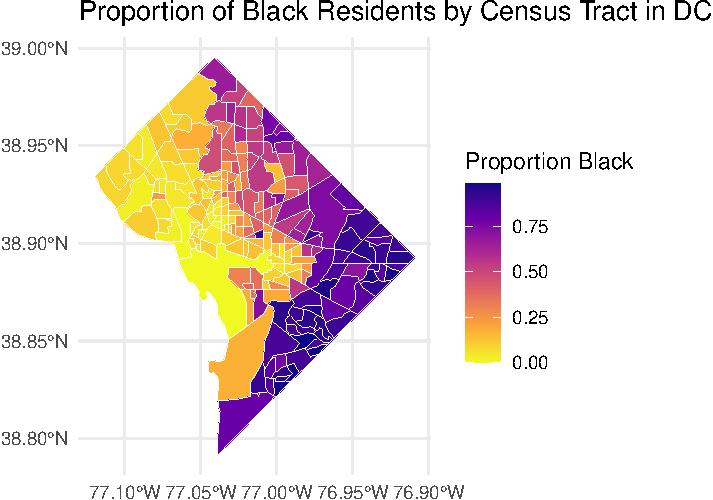
\includegraphics[keepaspectratio]{crit-comp-geo-pt1_files/figure-pdf/unnamed-chunk-15-1.pdf}}

\subsubsection{Is there a dividing
wall?}\label{is-there-a-dividing-wall}

Given that our model result indicate a significant measure of
segregation, we proceed with identifying the dividing wall. The maps we
have viewed up to this point give us a clear view of where that wall may
be.

\begin{Shaded}
\begin{Highlighting}[]
\NormalTok{dc\_combined }\OtherTok{\textless{}{-}}\NormalTok{ dc\_combined }\SpecialCharTok{\%\textgreater{}\%}
  \FunctionTok{mutate}\NormalTok{(}\AttributeTok{majority\_black =}\NormalTok{ proportion\_black }\SpecialCharTok{\textgreater{}} \FloatTok{0.5}\NormalTok{)}
\end{Highlighting}
\end{Shaded}

We'll join geometries by group.

\begin{Shaded}
\begin{Highlighting}[]
\CommentTok{\# Union geometries by group}
\NormalTok{union\_black }\OtherTok{\textless{}{-}}\NormalTok{ dc\_combined }\SpecialCharTok{\%\textgreater{}\%}
  \FunctionTok{filter}\NormalTok{(majority\_black) }\SpecialCharTok{\%\textgreater{}\%}
  \FunctionTok{summarise}\NormalTok{(}\AttributeTok{geometry =} \FunctionTok{st\_union}\NormalTok{(geometry))}

\NormalTok{union\_nonblack }\OtherTok{\textless{}{-}}\NormalTok{ dc\_combined }\SpecialCharTok{\%\textgreater{}\%}
  \FunctionTok{filter}\NormalTok{(}\SpecialCharTok{!}\NormalTok{majority\_black) }\SpecialCharTok{\%\textgreater{}\%}
  \FunctionTok{summarise}\NormalTok{(}\AttributeTok{geometry =} \FunctionTok{st\_union}\NormalTok{(geometry))}
\end{Highlighting}
\end{Shaded}

We then calculate boundary (difference) between groups (shared border).

\begin{Shaded}
\begin{Highlighting}[]
\NormalTok{boundary\_line }\OtherTok{=} 
  \FunctionTok{st\_intersection}\NormalTok{(}\FunctionTok{st\_boundary}\NormalTok{(union\_black), }\FunctionTok{st\_boundary}\NormalTok{(union\_nonblack))}
\end{Highlighting}
\end{Shaded}

We then plot the base polygons for the dividing wall.

\begin{Shaded}
\begin{Highlighting}[]
\FunctionTok{ggplot}\NormalTok{() }\SpecialCharTok{+}
  \FunctionTok{geom\_sf}\NormalTok{(}\AttributeTok{data =}\NormalTok{ dc\_combined, }\FunctionTok{aes}\NormalTok{(}\AttributeTok{fill =}\NormalTok{ majority\_black), }
          \AttributeTok{color =} \StringTok{"grey40"}\NormalTok{, }
          \AttributeTok{alpha =} \FloatTok{0.5}\NormalTok{) }\SpecialCharTok{+}
  \FunctionTok{geom\_sf}\NormalTok{(}\AttributeTok{data =}\NormalTok{ boundary\_line, }
          \AttributeTok{color =} \StringTok{"red"}\NormalTok{, }
          \AttributeTok{size =} \DecValTok{1}\NormalTok{) }\SpecialCharTok{+}
  \FunctionTok{labs}\NormalTok{(}\AttributeTok{title =} \StringTok{"Dividing Wall Between Majority Black and Non{-}Black Areas"}\NormalTok{) }\SpecialCharTok{+}
  \FunctionTok{theme\_minimal}\NormalTok{()}
\end{Highlighting}
\end{Shaded}

\pandocbounded{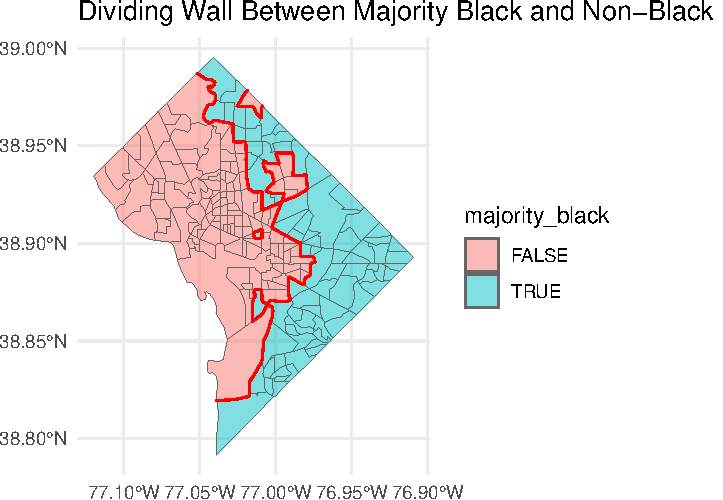
\includegraphics[keepaspectratio]{crit-comp-geo-pt1_files/figure-pdf/unnamed-chunk-19-1.pdf}}

\subsection{NC}\label{nc}

DC is a speical case since it is a city-state.

For NC, we'll use \texttt{geography\ =\ "county"} and then search for
those counties with higher values of segregation, and then we'll use
those ordered values to identify significant segregation and identify
potential dividing walls.

\begin{Shaded}
\begin{Highlighting}[]
\NormalTok{nc\_black\_pop }\OtherTok{\textless{}{-}} \FunctionTok{get\_acs}\NormalTok{(}
  \AttributeTok{geography =} \StringTok{"county"}\NormalTok{,}
  \AttributeTok{variables =} \StringTok{"B02001\_003"}\NormalTok{, }\CommentTok{\# Black/African American alone}
  \AttributeTok{state =} \StringTok{"NC"}\NormalTok{,}
  \AttributeTok{year =} \DecValTok{2023}\NormalTok{,}
  \AttributeTok{geometry =}\NormalTok{ T}
\NormalTok{)}
\end{Highlighting}
\end{Shaded}

\begin{Shaded}
\begin{Highlighting}[]
\FunctionTok{head}\NormalTok{(nc\_black\_pop)}
\end{Highlighting}
\end{Shaded}

\begin{verbatim}
Simple feature collection with 6 features and 5 fields
Geometry type: MULTIPOLYGON
Dimension:     XY
Bounding box:  xmin: -83.95288 ymin: 34.44087 xmax: -75.77333 ymax: 36.58812
Geodetic CRS:  NAD83
  GEOID                               NAME   variable estimate  moe
1 37133      Onslow County, North Carolina B02001_003    26157 1219
2 37009        Ashe County, North Carolina B02001_003      289  100
3 37169      Stokes County, North Carolina B02001_003     1543  373
4 37053   Currituck County, North Carolina B02001_003     1509  137
5 37173       Swain County, North Carolina B02001_003      212  112
6 37131 Northampton County, North Carolina B02001_003     9451  187
                        geometry
1 MULTIPOLYGON (((-77.17131 3...
2 MULTIPOLYGON (((-81.74065 3...
3 MULTIPOLYGON (((-80.4502 36...
4 MULTIPOLYGON (((-76.3133 36...
5 MULTIPOLYGON (((-83.94939 3...
6 MULTIPOLYGON (((-77.89977 3...
\end{verbatim}

We'll then plot our data to make sure that our map features are working
properly.

\begin{Shaded}
\begin{Highlighting}[]
\FunctionTok{ggplot}\NormalTok{(nc\_black\_pop) }\SpecialCharTok{+}
  \FunctionTok{geom\_sf}\NormalTok{(}\FunctionTok{aes}\NormalTok{(}\AttributeTok{fill =}\NormalTok{ estimate)) }\SpecialCharTok{+}
  \FunctionTok{scale\_fill\_viridis\_c}\NormalTok{(}\AttributeTok{option =} \StringTok{"magma"}\NormalTok{, }
                       \AttributeTok{na.value =} \StringTok{"grey50"}\NormalTok{) }\SpecialCharTok{+}
  \FunctionTok{labs}\NormalTok{(}\AttributeTok{title =} \StringTok{"Estimated Black Population by County in NC (2023)"}\NormalTok{,}
       \AttributeTok{fill =} \StringTok{"Population"}\NormalTok{) }\SpecialCharTok{+}
  \FunctionTok{theme\_minimal}\NormalTok{()}
\end{Highlighting}
\end{Shaded}

\pandocbounded{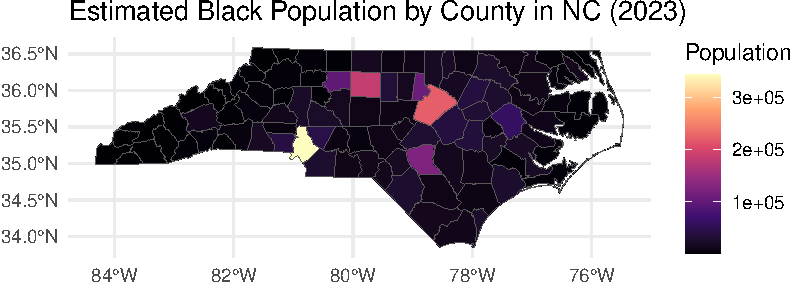
\includegraphics[keepaspectratio]{crit-comp-geo-pt1_files/figure-pdf/unnamed-chunk-22-1.pdf}}

\begin{Shaded}
\begin{Highlighting}[]
\FunctionTok{ggplot}\NormalTok{(nc\_black\_pop) }\SpecialCharTok{+}
  \FunctionTok{geom\_sf}\NormalTok{(}\FunctionTok{aes}\NormalTok{(}\AttributeTok{fill =}\NormalTok{ estimate)) }\SpecialCharTok{+}
  \FunctionTok{scale\_fill\_viridis\_c}\NormalTok{(}\AttributeTok{option =} \StringTok{"magma"}\NormalTok{, }
                       \AttributeTok{na.value =} \StringTok{"grey50"}\NormalTok{,}
                       \AttributeTok{labels =}\NormalTok{ comma) }\SpecialCharTok{+}
  \FunctionTok{labs}\NormalTok{(}\AttributeTok{title =} \StringTok{"Estimated Black Population by County in NC (2023)"}\NormalTok{,}
       \AttributeTok{fill =} \StringTok{"Population"}\NormalTok{) }\SpecialCharTok{+}
  \FunctionTok{theme\_minimal}\NormalTok{()}
\end{Highlighting}
\end{Shaded}

\pandocbounded{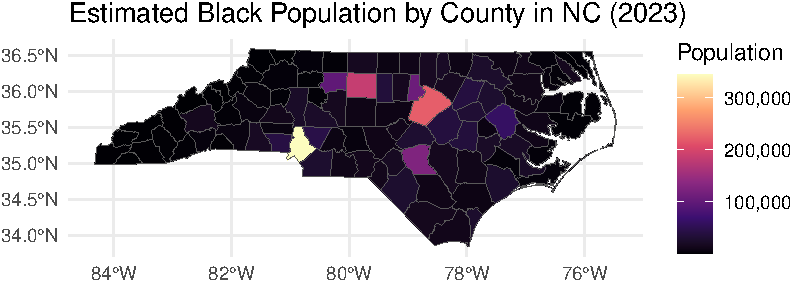
\includegraphics[keepaspectratio]{crit-comp-geo-pt1_files/figure-pdf/unnamed-chunk-23-1.pdf}}

\newpage

\section{References}\label{references}

\href{}{Hudson, P. J., \& McKittrick, K. (2014). The geographies of
blackness and anti-blackness. \emph{The CLR James Journal, 20}(1/2),
233--240.}

\href{}{King, T. L., Navarro, J., \& Smith, A. (2020). \emph{Otherwise
worlds: Against settler colonialism and anti-blackness}. Duke University
Press.}

\href{}{Lu, B., Harris, P., Charlton, M., \& Brunsdon, C. (2014). The
GWmodel R package: Further topics for exploring spatial heterogeneity
using geographically weighted models. \emph{Geo-Spatial Information
Science, 17}(2), 85--101.}

\href{}{Sørensen, A. B. (1978). Mathematical models in sociology.
\emph{Annual Review of Sociology, 4}, 345--371.}

\href{}{Walker, K. (2023). \emph{Analyzing us census data: Methods,
maps, and models in R}. Chapman.}

\newpage

\section{Coda}\label{coda}

While the index of dissimilarity offers a clear and interpretable
measure of segregation, it is only one facet of complex social dynamics.
Future work could extend this analysis by incorporating:

\begin{itemize}
\tightlist
\item
  Isolation and clustering indices to capture different aspects of
  segregation.
\item
  Temporal dynamics to assess how patterns shift over time.
\item
  Qualitative data integration to contextualize spatial patterns with
  lived experiences.
\item
  Policy evaluation assessing impacts of urban planning and housing
  initiatives.
\end{itemize}

This technical file lays the foundation for quantitative historical
geography research by demonstrating reproducible workflows with open
Census data and modern R tools. The methodologies presented can be
readily adapted to other metropolitan areas and demographic groups for
comparative analyses.

Continued interdisciplinary collaboration will deepen our understanding
of spatial inequality and support informed efforts to foster equitable
communities.

Document No: 20250922-na




\end{document}
